\documentclass[conference]{IEEEtran}
\IEEEoverridecommandlockouts
\usepackage{cite}
\usepackage{amsmath,amssymb,amsfonts}
\usepackage{graphicx}
\usepackage{float}
\usepackage{xcolor}
\usepackage{booktabs}
\usepackage{tikz}
\usetikzlibrary{arrows.meta,positioning,fit,backgrounds}
\usepackage{url}

\def\BibTeX{{\rm B\kern-.05em{\sc i\kern-.025em b}\kern-.08em
    T\kern-.1667em\lower.7ex\hbox{E}\kern-.125emX}}
\begin{document}

\title{An Auditable LLM Gating Agent for Poisoning-Resilient Federated IoT Security}

\author{\IEEEauthorblockN{Aashma Uprety, \textit{Student Member, IEEE} and Danda B. Rawat, \textit{Senior Member, IEEE}}
\IEEEauthorblockA{Department of Electrical Engineering and Computer Science, Howard University, Washington, DC, USA\\
aashma.uprety@bison.howard.edu, db.rawat@ieee.org}
}

\maketitle

\begin{abstract}
Federated learning (FL) is often treated as private and secure by default for IoT device identification and intrusion detection, but standard aggregation offers no defense against a compromised participant, and no prior work evaluates poisoning risk for both tasks, though we test each separately, not as one jointly-attacked model. Plain FedAvg's accuracy collapses under realistic poisoning for device identification (0.828 to 0.038 macro-F1), just as for intrusion detection. We then evaluate an LLM-based reasoning agent, the \emph{Gating Agent}, that reviews every client update and decides to accept, downweight, or exclude it with a plain-language rationale, in place of a fixed statistical rule, against untargeted, targeted, and delayed "trust-building" poisoning. An 8B open model fails this judgment outright (0.06--0.24 macro-F1); a 14B model, once its evidence is designed correctly, reaches 0.896--0.997 across two real IoT datasets and three attack types, matching or exceeding a rule-based reference on every tested configuration. A fast, non-LLM clustering baseline matches this accuracy at a fraction of the cost, so we position auditability as the agent's hypothesized advantage, not yet validated with human evaluators, and introduce a selective variant that halves the LLM's measured cost -- a design that itself failed once, was diagnosed, and fixed, reported rather than hidden. Against every attacker we tested, none found an edge. Code and full results are public: \url{https://github.com/aashmauprety/fediot-gating-agent}.
\end{abstract}

\begin{IEEEkeywords}
Federated Learning, Internet of Things, Large Language Models, Agentic AI, Robust Aggregation, Network Security
\end{IEEEkeywords}

\section{Introduction}
IoT gateways increasingly use federated learning (FL) to train device-identification and intrusion-detection models without centralizing raw traffic. FL keeps data local, but it is not a security mechanism on its own: a compromised gateway can submit a poisoned update, and standard aggregation (FedAvg \cite{mcmahan2017communication}) has no defense against this. Byzantine-robust rules such as trimmed-mean/median \cite{yin2018byzantine} and Krum \cite{blanchard2017machine} catch statistically anomalous updates, but they apply a fixed threshold and cannot explain, in terms an operator can audit, why a given client was excluded.

We evaluate a different design: a single LLM-based reasoning agent, the \emph{Gating Agent}, that reviews each client's update every round against an explicit threat model and decides to accept, downweight, or exclude it, with a natural-language rationale instead of a bare statistical flag. This is close in spirit to recent LLM-agent work for network intrusion detection \cite{islam2026maids,jamshidi2026trillm}, which shows LLM reasoning can catch what fixed thresholds miss but leaves open whether a real model works for this decision, and at what scale -- we answer both, with real attacks on real IoT traffic.

This paper makes four contributions. First, plain FL degrades under realistic poisoning for both device identification and intrusion detection -- two separate experiments on the same shared-encoder architecture, not one jointly-attacked multi-task model -- a combination no prior FL device-ID or FL-IDS work evaluates (Table \ref{tab:coverage}). Second, we validate the LLM-based Gating Agent against the tested attacks, diagnosing and fixing five real failure modes, and measure a capability boundary. Third, we test against a fast non-LLM baseline and independent and colluding adaptive attackers, and introduce a selective variant halving the LLM's cost -- itself requiring a real bug found and fixed. Fourth, we measure real per-decision latency and resource cost directly, not aggregate totals.

\section{Related Work}
\label{sec:relwork}
IoT device identification and intrusion detection have been studied extensively but mostly separately, and mostly with centralized, hand-crafted-feature pipelines \cite{meidan2017profiliot}, which do not generalize across deployments without re-engineering. Self-supervised traffic representations improve generalization but remain centralized \cite{sivanathan2026generalizable}.

Within federated device identification, ConFedDI \cite{chen2025confeddi} and FGLIoT \cite{wang2025fgliot} report 99.4--99.8\% F1 -- higher than our 0.792 on UNSW, but closed-set, no zero-shot onboarding. He et al. \cite{he2021edge} identify edge devices federatedly, closest to our setup, with no threat model at all. S\'anchez S\'anchez et al. \cite{sanchez2021robust} consider poisoning for federated device-ID (hardware features, not network traffic, no IDS component) -- not unprecedented alone, but not combined with intrusion detection as we do.

Within federated IDS with an explicit robustness mechanism, FedMADE \cite{sun2024fedmade} clusters by class-probability matrix but does not test an adaptive attacker. FedKD-IDS \cite{fedkdids2025} defends N-BaIoT via knowledge-distillation voting with a weaker backbone. AGAT-FL \cite{sanjalawe2025agatfl} combines graph attention with Mahalanobis filtering -- the same family as GShield \cite{sameera2025gshield}, confirming clustering, not an LLM, is the dominant non-LLM defense here, the family we benchmark in Section \ref{sec:results}.

On the security side, FL is vulnerable to model- and data-poisoning \cite{lyu2020threats,bagdasaryan2020backdoor}, and Byzantine-robust rules such as trimmed-mean/median \cite{yin2018byzantine} and Krum \cite{blanchard2017machine} defend with fixed thresholds that cannot explain a given exclusion to an operator. Recent work applies LLM agents to network security: retrieval-augmented multi-agent intrusion detection \cite{islam2026maids} and multi-model trust-weighted voting across federated participants \cite{jamshidi2026trillm}, the latter explicitly flagging long-term, consistency-aware trust modeling as open future work, which our Bayesian long-term prior addresses directly. A discounted Beta-reputation posterior for decentralized Byzantine-resilient FL trust has also been proposed independently \cite{jia2026openclaw}; our contribution is not the Beta posterior but pairing it with an LLM reasoning in natural language over its value, not a fixed reputation rule. Closest in spirit is Jamshidi et al. \cite{jamshidi2026thinkfast}, an edge-only, non-federated IDS where local classifiers detect anomalies and an LLM enriches the alert afterward -- their LLM explains an already-fixed verdict rather than making it, and their future work lists adversarial robustness as untested. Our LLM's output is not bolted onto a fixed decision -- it is the decision, tested against real poisoning attacks.

A raw-accuracy comparison against Table \ref{tab:coverage}'s prior work would not be meaningful -- each reports its own number on its own dataset, so cross-row ranking would be an apples-to-oranges artifact. What is comparable is capability coverage: no prior system combines federated device-ID and IDS on one shared encoder, validates an LLM making the actual per-round aggregation decision against real poisoning attacks, and measures whether model scale is a hard requirement for it.

\begin{table}[t]
\centering
\scriptsize
\caption{Capability coverage vs. the closest prior work (not an accuracy comparison -- see text).}
\label{tab:coverage}
\begin{tabular}{@{}lccccc@{}}
\toprule
\textbf{Work} & \textbf{Dev-ID} & \textbf{IDS} & \textbf{Pois.} & \textbf{Audit} & \textbf{0-shot} \\
\midrule
ConFedDI/FGLIoT/He \cite{chen2025confeddi,wang2025fgliot,he2021edge} & \checkmark & & & & \\
S\'anchez S\'anchez \cite{sanchez2021robust} & \checkmark & & \checkmark & & \\
FedMADE \cite{sun2024fedmade} & & \checkmark & & & \\
FedKD-IDS \cite{fedkdids2025} & & \checkmark & \checkmark & & \\
AGAT-FL / GShield \cite{sanjalawe2025agatfl,sameera2025gshield} & & \checkmark & \checkmark & & \\
MAIDS \cite{islam2026maids} & & \checkmark & & & \\
Tri-LLM \cite{jamshidi2026trillm} & & \checkmark & & & \\
Think Fast \cite{jamshidi2026thinkfast} & & \checkmark & $\ast$ & \checkmark & \\
\textbf{This work} & \checkmark & \checkmark & \checkmark & \checkmark & \checkmark \\
\bottomrule
\end{tabular}
\\[2pt]
{\scriptsize $\ast$ Not federated by design, so FL-aggregation poisoning is out of scope, not tested-and-absent; its own reported future work lists adversarial robustness as untested.}
\end{table}

\section{System and Threat Model}
We consider $N$ gateway clients training a shared classifier federatedly; each round, the server aggregates updates via FedAvg \cite{mcmahan2017communication} unless a defense intervenes. The server is honest-but-curious; a fully malicious server is out of scope. Gating requires the server (and LLM) to observe each client's digest -- compatible with honest-but-curious, but not secure aggregation, which would hide these signals; combining the two is open. Up to a fraction $\alpha$ of clients may be compromised: a compromised client can mislabel local data or submit an arbitrary update, may collude with others, and may control \emph{when} it deviates from honest behavior rather than following a fixed schedule.

We evaluate three adversary goals. \textbf{Untargeted}: degrade overall model accuracy (e.g.\ random label-flipping). \textbf{Targeted}: cause one specific class to be systematically misclassified as another, attacker-chosen class. \textbf{Trust-building (delayed)}: behave honestly for $D$ rounds specifically to build up a favorable trust history, then switch to an untargeted or targeted attack -- an attack that exists only because a long-term trust mechanism exists to exploit.

\subsection{The Gating Agent}
Fig.~\ref{system} shows the overall system this design defends. Each round, the server computes a compact \emph{digest} $g_n^{(r)}$ per client $n$: the update norm, its cosine similarity to the previous round's aggregated update, and a calibration-loss delta on a held-out set. A per-client Bayesian long-term trust posterior $\mathrm{Beta}(\alpha_n,\beta_n)$ \cite{josang2002beta} tracks $n$'s history of non-anomalous participation, updated each round with the gating score as a soft observation. The Gating Agent -- an LLM given this round's digest and, when needed, the long-term posterior -- outputs a gating score $\tau_n^{(r)} \in [0,1]$ and an action in \{accept, downweight, exclude\}, with a rationale naming the evidence behind it. FedAvg is then applied with weights $\tau_n^{(r)}$ in place of uniform $1/N$, so an excluded update contributes nothing and a downweighted one contributes partially.

The design choice that matters most is \emph{where state lives}. An LLM tracking long-term trust in its own context tends to react to each round's surface anomaly rather than weighing accumulated history, since chain-of-thought accumulates text, not probability mass. We keep the Bayesian posterior and the final decision fully external and deterministic, giving the LLM exactly one job: judge how anomalous the current digest looks, in isolation -- substituting for a fixed z-score threshold, with everything downstream outside the LLM's control.

A real trace makes this concrete (round 22 of a $D{=}20$ trust-building run, three malicious clients mid-attack): client\_0 and client\_2 both get "both z-scores are far from zero and calibration loss significantly worsened" $\to$ exclude (0.0); client\_1 gets the identical rationale plus "long-term posterior mean=0.74 over 9 rounds downgrades exclude to downweight" $\to$ downweight (0.5). Two clients with the same evidence get excluded outright; the third gets a lighter penalty purely because its own accumulated history earns partial benefit of the doubt -- an operator can audit exactly why three otherwise-identical rounds resolved differently.

\begin{figure*}[t]
    \centering
    \resizebox{\textwidth}{!}{% FedIoT-Gate system diagram (TikZ), with Font Awesome Free icon badges
% (CC BY 4.0, https://fontawesome.com/license/free) for visual clarity.
% Three stages, left to right:
%   (1) Phase 0 -- federated self-supervised encoder pretraining
%   (2) Phase I -- digest-gated federated classifier training
%   (3) Zero-shot onboarding of a new device type via the Gating Agent
%
% Intended usage from main.tex (requires \usepackage{tikz,graphicx} with
% the libraries listed below loaded in the preamble):
%
%   \begin{figure*}[t]
%       \centering
%       \resizebox{\textwidth}{!}{% FedIoT-Gate system diagram (TikZ), with Font Awesome Free icon badges
% (CC BY 4.0, https://fontawesome.com/license/free) for visual clarity.
% Three stages, left to right:
%   (1) Phase 0 -- federated self-supervised encoder pretraining
%   (2) Phase I -- digest-gated federated classifier training
%   (3) Zero-shot onboarding of a new device type via the Gating Agent
%
% Intended usage from main.tex (requires \usepackage{tikz,graphicx} with
% the libraries listed below loaded in the preamble):
%
%   \begin{figure*}[t]
%       \centering
%       \resizebox{\textwidth}{!}{% FedIoT-Gate system diagram (TikZ), with Font Awesome Free icon badges
% (CC BY 4.0, https://fontawesome.com/license/free) for visual clarity.
% Three stages, left to right:
%   (1) Phase 0 -- federated self-supervised encoder pretraining
%   (2) Phase I -- digest-gated federated classifier training
%   (3) Zero-shot onboarding of a new device type via the Gating Agent
%
% Intended usage from main.tex (requires \usepackage{tikz,graphicx} with
% the libraries listed below loaded in the preamble):
%
%   \begin{figure*}[t]
%       \centering
%       \resizebox{\textwidth}{!}{\input{figures/system-diagram/gating_system_diagram.tex}}
%       \caption{...}
%       \label{system}
%   \end{figure*}
%
% Icon PDFs: figures/system-diagram/icons/*.pdf (paths relative to
% main.tex's directory). Can also be compiled on its own via
% figures/system-diagram/standalone.tex.

\newcommand{\sysicon}[1]{\includegraphics[height=0.38cm]{figures/system-diagram/icons/#1.pdf}}

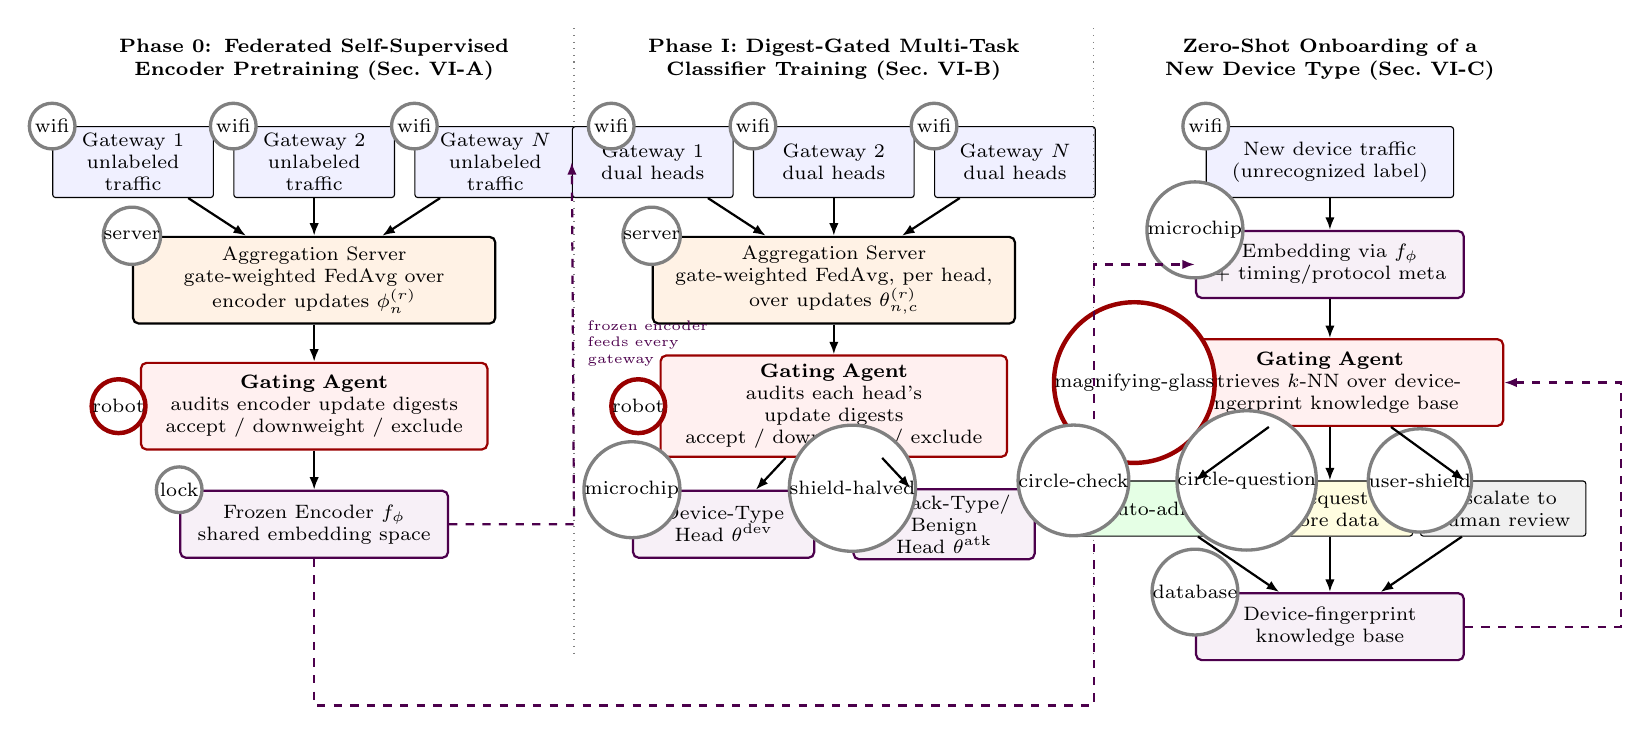
\begin{tikzpicture}[
    font=\scriptsize,
    gateway/.style={rectangle, draw, rounded corners=1pt, fill=blue!6,
        minimum width=2.0cm, minimum height=0.9cm, text width=1.9cm, align=center, inner sep=2pt},
    server/.style={rectangle, draw, thick, rounded corners=2pt, fill=orange!10,
        minimum width=4.6cm, minimum height=1.1cm, text width=4.3cm, align=center, inner sep=3pt},
    agent/.style={rectangle, draw=red!60!black, thick, rounded corners=2pt, fill=red!6,
        minimum width=4.4cm, minimum height=1.1cm, text width=4.1cm, align=center, inner sep=3pt},
    frozen/.style={rectangle, draw=violet!60!black, thick, rounded corners=2pt, fill=violet!6,
        minimum width=3.4cm, minimum height=0.85cm, text width=3.1cm, align=center, inner sep=2pt},
    head/.style={rectangle, draw=violet!60!black, thick, rounded corners=2pt, fill=violet!6,
        minimum width=2.3cm, minimum height=0.85cm, text width=2.0cm, align=center, inner sep=2pt},
    decision/.style={rectangle, draw, rounded corners=1pt, minimum width=2.1cm,
        minimum height=0.7cm, text width=1.9cm, align=center, inner sep=2pt},
    stagetitle/.style={font=\bfseries\scriptsize, align=center, text width=6.0cm},
    arr/.style={-{Latex[length=1.6mm]}, thick},
    dashedarr/.style={-{Latex[length=1.6mm]}, thick, dashed, violet!60!black},
    badge/.style={circle, draw=black!50, very thick, fill=white, minimum size=0.58cm, inner sep=0pt},
    agentbadge/.style={circle, draw=red!60!black, ultra thick, fill=white, minimum size=0.62cm, inner sep=0pt},
]

%% ================= Stage 1 (centered at x=0): Phase 0 =================
\node[stagetitle] (s1title) at (0,3.3) {Phase 0: Federated Self-Supervised Encoder Pretraining (Sec.~VI-A)};

\node[gateway] (g1a) at (-2.3,2.0) {Gateway 1\\ unlabeled traffic};
\node[gateway] (g1b) at (0,2.0)    {Gateway 2\\ unlabeled traffic};
\node[gateway] (g1c) at (2.3,2.0)  {Gateway $N$\\ unlabeled traffic};
\node[badge] at (g1a.north west) {\sysicon{wifi}};
\node[badge] at (g1b.north west) {\sysicon{wifi}};
\node[badge] at (g1c.north west) {\sysicon{wifi}};

\node[server] (srv1) at (0,0.5) {Aggregation Server\\ gate-weighted FedAvg over\\ encoder updates $\phi_n^{(r)}$};
\node[badge] at (srv1.north west) {\sysicon{server}};
\node[agent] (agent1) at (0,-1.1) {\textbf{Gating Agent}\\ audits encoder update digests\\ accept / downweight / exclude};
\node[agentbadge] at ([xshift=-0.27cm]agent1.west) {\sysicon{robot}};
\node[frozen] (frozenenc) at (0,-2.6) {Frozen Encoder $f_\phi$\\ shared embedding space};
\node[badge] at (frozenenc.north west) {\sysicon{lock}};

\draw[arr] (g1a) -- (srv1);
\draw[arr] (g1b) -- (srv1);
\draw[arr] (g1c) -- (srv1);
\draw[arr] (srv1) -- (agent1);
\draw[arr] (agent1) -- (frozenenc);

%% ---------- divider 1 ----------
\draw[dotted, gray] (3.3,3.7) -- (3.3,-4.3);

%% ================= Stage 2 (centered at x=6.6): Phase I =================
\node[stagetitle] (s2title) at (6.6,3.3) {Phase I: Digest-Gated Multi-Task Classifier Training (Sec.~VI-B)};

\node[gateway] (g2a) at (4.3,2.0) {Gateway 1\\ dual heads};
\node[gateway] (g2b) at (6.6,2.0) {Gateway 2\\ dual heads};
\node[gateway] (g2c) at (8.9,2.0) {Gateway $N$\\ dual heads};
\node[badge] at ([xshift=0.5cm]g2a.north west) {\sysicon{wifi}};
\node[badge] at (g2b.north west) {\sysicon{wifi}};
\node[badge] at (g2c.north west) {\sysicon{wifi}};

\node[server] (srv2) at (6.6,0.5) {Aggregation Server\\ gate-weighted FedAvg, per head,\\ over updates $\theta_{n,c}^{(r)}$};
\node[badge] at (srv2.north west) {\sysicon{server}};
\node[agent] (agent2) at (6.6,-1.1) {\textbf{Gating Agent}\\ audits each head's update digests\\ accept / downweight / exclude};
\node[agentbadge] at ([xshift=-0.27cm]agent2.west) {\sysicon{robot}};
\node[head] (devclf) at (5.2,-2.6) {Device-Type\\ Head $\theta^{\text{dev}}$};
\node[head] (atkclf) at (8.0,-2.6) {Attack-Type/\\ Benign Head $\theta^{\text{atk}}$};
\node[badge] at (devclf.north west) {\sysicon{microchip}};
\node[badge] at (atkclf.north west) {\sysicon{shield-halved}};

\draw[arr] (g2a) -- (srv2);
\draw[arr] (g2b) -- (srv2);
\draw[arr] (g2c) -- (srv2);
\draw[arr] (srv2) -- (agent2);
\draw[arr] (agent2) -- (devclf);
\draw[arr] (agent2) -- (atkclf);

\draw[dashedarr] (frozenenc.east) -- (3.3,-2.6) -- (g2a.west);
\node[font=\tiny, align=left, violet!60!black, anchor=west, text width=1.7cm] at (3.35,-0.3) {frozen encoder\\ feeds every\\ gateway};

%% ---------- divider 2 ----------
\draw[dotted, gray] (9.9,3.7) -- (9.9,-4.3);

%% ================= Stage 3 (centered at x=12.9): Onboarding =================
\node[stagetitle] (s3title) at (12.9,3.3) {Zero-Shot Onboarding of a New Device Type (Sec.~VI-C)};

\node[gateway, text width=3.0cm, minimum width=3.1cm] (newdev) at (12.9,2.0) {New device traffic\\ (unrecognized label)};
\node[badge] at (newdev.north west) {\sysicon{wifi}};
\node[frozen] (embnew) at (12.9,0.7) {Embedding via $f_\phi$\\ + timing/protocol meta};
\node[badge] at (embnew.north west) {\sysicon{microchip}};
\node[agent] (agent3) at (12.9,-0.8) {\textbf{Gating Agent}\\ retrieves $k$-NN over device-\\ fingerprint knowledge base};
\node[agentbadge] at ([xshift=-0.27cm]agent3.west) {\sysicon{magnifying-glass}};

\draw[arr] (newdev) -- (embnew);
\draw[arr] (embnew) -- (agent3);
\draw[dashedarr] (frozenenc.south) -- (0,-4.9) -- (9.9,-4.9) -- (9.9,0.7) -- (embnew.west);

\node[decision, fill=green!10] (admit) at (10.7,-2.4) {Auto-admit};
\node[decision, fill=yellow!12] (defer) at (12.9,-2.4) {Request\\ more data};
\node[decision, fill=gray!12] (escalate) at (15.1,-2.4) {Escalate to\\ human review};
\node[badge] at (admit.north west) {\sysicon{circle-check}};
\node[badge] at (defer.north west) {\sysicon{circle-question}};
\node[badge] at (escalate.north west) {\sysicon{user-shield}};

\draw[arr] (agent3) -- (admit);
\draw[arr] (agent3) -- (defer);
\draw[arr] (agent3) -- (escalate);

\node[frozen] (kb) at (12.9,-3.9) {Device-fingerprint\\ knowledge base};
\node[badge] at (kb.north west) {\sysicon{database}};
\draw[arr] (admit) -- (kb);
\draw[arr] (defer) -- (kb);
\draw[arr] (escalate) -- (kb);
\draw[dashedarr] (kb.east) -- (16.6,-3.9) -- (16.6,-0.8) -- (agent3.east);

\end{tikzpicture}
}
%       \caption{...}
%       \label{system}
%   \end{figure*}
%
% Icon PDFs: figures/system-diagram/icons/*.pdf (paths relative to
% main.tex's directory). Can also be compiled on its own via
% figures/system-diagram/standalone.tex.

\newcommand{\sysicon}[1]{\includegraphics[height=0.38cm]{figures/system-diagram/icons/#1.pdf}}

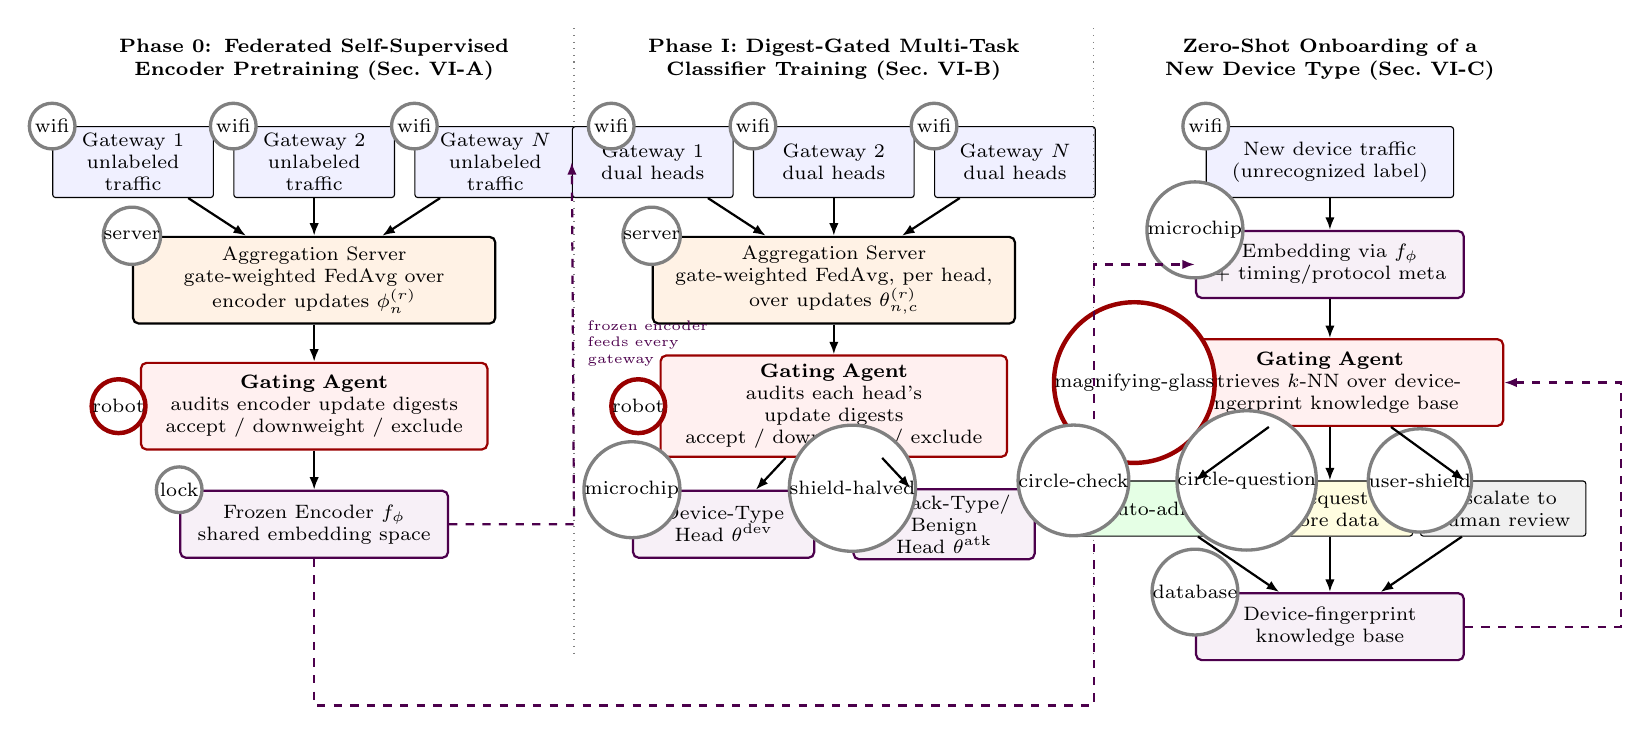
\begin{tikzpicture}[
    font=\scriptsize,
    gateway/.style={rectangle, draw, rounded corners=1pt, fill=blue!6,
        minimum width=2.0cm, minimum height=0.9cm, text width=1.9cm, align=center, inner sep=2pt},
    server/.style={rectangle, draw, thick, rounded corners=2pt, fill=orange!10,
        minimum width=4.6cm, minimum height=1.1cm, text width=4.3cm, align=center, inner sep=3pt},
    agent/.style={rectangle, draw=red!60!black, thick, rounded corners=2pt, fill=red!6,
        minimum width=4.4cm, minimum height=1.1cm, text width=4.1cm, align=center, inner sep=3pt},
    frozen/.style={rectangle, draw=violet!60!black, thick, rounded corners=2pt, fill=violet!6,
        minimum width=3.4cm, minimum height=0.85cm, text width=3.1cm, align=center, inner sep=2pt},
    head/.style={rectangle, draw=violet!60!black, thick, rounded corners=2pt, fill=violet!6,
        minimum width=2.3cm, minimum height=0.85cm, text width=2.0cm, align=center, inner sep=2pt},
    decision/.style={rectangle, draw, rounded corners=1pt, minimum width=2.1cm,
        minimum height=0.7cm, text width=1.9cm, align=center, inner sep=2pt},
    stagetitle/.style={font=\bfseries\scriptsize, align=center, text width=6.0cm},
    arr/.style={-{Latex[length=1.6mm]}, thick},
    dashedarr/.style={-{Latex[length=1.6mm]}, thick, dashed, violet!60!black},
    badge/.style={circle, draw=black!50, very thick, fill=white, minimum size=0.58cm, inner sep=0pt},
    agentbadge/.style={circle, draw=red!60!black, ultra thick, fill=white, minimum size=0.62cm, inner sep=0pt},
]

%% ================= Stage 1 (centered at x=0): Phase 0 =================
\node[stagetitle] (s1title) at (0,3.3) {Phase 0: Federated Self-Supervised Encoder Pretraining (Sec.~VI-A)};

\node[gateway] (g1a) at (-2.3,2.0) {Gateway 1\\ unlabeled traffic};
\node[gateway] (g1b) at (0,2.0)    {Gateway 2\\ unlabeled traffic};
\node[gateway] (g1c) at (2.3,2.0)  {Gateway $N$\\ unlabeled traffic};
\node[badge] at (g1a.north west) {\sysicon{wifi}};
\node[badge] at (g1b.north west) {\sysicon{wifi}};
\node[badge] at (g1c.north west) {\sysicon{wifi}};

\node[server] (srv1) at (0,0.5) {Aggregation Server\\ gate-weighted FedAvg over\\ encoder updates $\phi_n^{(r)}$};
\node[badge] at (srv1.north west) {\sysicon{server}};
\node[agent] (agent1) at (0,-1.1) {\textbf{Gating Agent}\\ audits encoder update digests\\ accept / downweight / exclude};
\node[agentbadge] at ([xshift=-0.27cm]agent1.west) {\sysicon{robot}};
\node[frozen] (frozenenc) at (0,-2.6) {Frozen Encoder $f_\phi$\\ shared embedding space};
\node[badge] at (frozenenc.north west) {\sysicon{lock}};

\draw[arr] (g1a) -- (srv1);
\draw[arr] (g1b) -- (srv1);
\draw[arr] (g1c) -- (srv1);
\draw[arr] (srv1) -- (agent1);
\draw[arr] (agent1) -- (frozenenc);

%% ---------- divider 1 ----------
\draw[dotted, gray] (3.3,3.7) -- (3.3,-4.3);

%% ================= Stage 2 (centered at x=6.6): Phase I =================
\node[stagetitle] (s2title) at (6.6,3.3) {Phase I: Digest-Gated Multi-Task Classifier Training (Sec.~VI-B)};

\node[gateway] (g2a) at (4.3,2.0) {Gateway 1\\ dual heads};
\node[gateway] (g2b) at (6.6,2.0) {Gateway 2\\ dual heads};
\node[gateway] (g2c) at (8.9,2.0) {Gateway $N$\\ dual heads};
\node[badge] at ([xshift=0.5cm]g2a.north west) {\sysicon{wifi}};
\node[badge] at (g2b.north west) {\sysicon{wifi}};
\node[badge] at (g2c.north west) {\sysicon{wifi}};

\node[server] (srv2) at (6.6,0.5) {Aggregation Server\\ gate-weighted FedAvg, per head,\\ over updates $\theta_{n,c}^{(r)}$};
\node[badge] at (srv2.north west) {\sysicon{server}};
\node[agent] (agent2) at (6.6,-1.1) {\textbf{Gating Agent}\\ audits each head's update digests\\ accept / downweight / exclude};
\node[agentbadge] at ([xshift=-0.27cm]agent2.west) {\sysicon{robot}};
\node[head] (devclf) at (5.2,-2.6) {Device-Type\\ Head $\theta^{\text{dev}}$};
\node[head] (atkclf) at (8.0,-2.6) {Attack-Type/\\ Benign Head $\theta^{\text{atk}}$};
\node[badge] at (devclf.north west) {\sysicon{microchip}};
\node[badge] at (atkclf.north west) {\sysicon{shield-halved}};

\draw[arr] (g2a) -- (srv2);
\draw[arr] (g2b) -- (srv2);
\draw[arr] (g2c) -- (srv2);
\draw[arr] (srv2) -- (agent2);
\draw[arr] (agent2) -- (devclf);
\draw[arr] (agent2) -- (atkclf);

\draw[dashedarr] (frozenenc.east) -- (3.3,-2.6) -- (g2a.west);
\node[font=\tiny, align=left, violet!60!black, anchor=west, text width=1.7cm] at (3.35,-0.3) {frozen encoder\\ feeds every\\ gateway};

%% ---------- divider 2 ----------
\draw[dotted, gray] (9.9,3.7) -- (9.9,-4.3);

%% ================= Stage 3 (centered at x=12.9): Onboarding =================
\node[stagetitle] (s3title) at (12.9,3.3) {Zero-Shot Onboarding of a New Device Type (Sec.~VI-C)};

\node[gateway, text width=3.0cm, minimum width=3.1cm] (newdev) at (12.9,2.0) {New device traffic\\ (unrecognized label)};
\node[badge] at (newdev.north west) {\sysicon{wifi}};
\node[frozen] (embnew) at (12.9,0.7) {Embedding via $f_\phi$\\ + timing/protocol meta};
\node[badge] at (embnew.north west) {\sysicon{microchip}};
\node[agent] (agent3) at (12.9,-0.8) {\textbf{Gating Agent}\\ retrieves $k$-NN over device-\\ fingerprint knowledge base};
\node[agentbadge] at ([xshift=-0.27cm]agent3.west) {\sysicon{magnifying-glass}};

\draw[arr] (newdev) -- (embnew);
\draw[arr] (embnew) -- (agent3);
\draw[dashedarr] (frozenenc.south) -- (0,-4.9) -- (9.9,-4.9) -- (9.9,0.7) -- (embnew.west);

\node[decision, fill=green!10] (admit) at (10.7,-2.4) {Auto-admit};
\node[decision, fill=yellow!12] (defer) at (12.9,-2.4) {Request\\ more data};
\node[decision, fill=gray!12] (escalate) at (15.1,-2.4) {Escalate to\\ human review};
\node[badge] at (admit.north west) {\sysicon{circle-check}};
\node[badge] at (defer.north west) {\sysicon{circle-question}};
\node[badge] at (escalate.north west) {\sysicon{user-shield}};

\draw[arr] (agent3) -- (admit);
\draw[arr] (agent3) -- (defer);
\draw[arr] (agent3) -- (escalate);

\node[frozen] (kb) at (12.9,-3.9) {Device-fingerprint\\ knowledge base};
\node[badge] at (kb.north west) {\sysicon{database}};
\draw[arr] (admit) -- (kb);
\draw[arr] (defer) -- (kb);
\draw[arr] (escalate) -- (kb);
\draw[dashedarr] (kb.east) -- (16.6,-3.9) -- (16.6,-0.8) -- (agent3.east);

\end{tikzpicture}
}
%       \caption{...}
%       \label{system}
%   \end{figure*}
%
% Icon PDFs: figures/system-diagram/icons/*.pdf (paths relative to
% main.tex's directory). Can also be compiled on its own via
% figures/system-diagram/standalone.tex.

\newcommand{\sysicon}[1]{\includegraphics[height=0.38cm]{figures/system-diagram/icons/#1.pdf}}

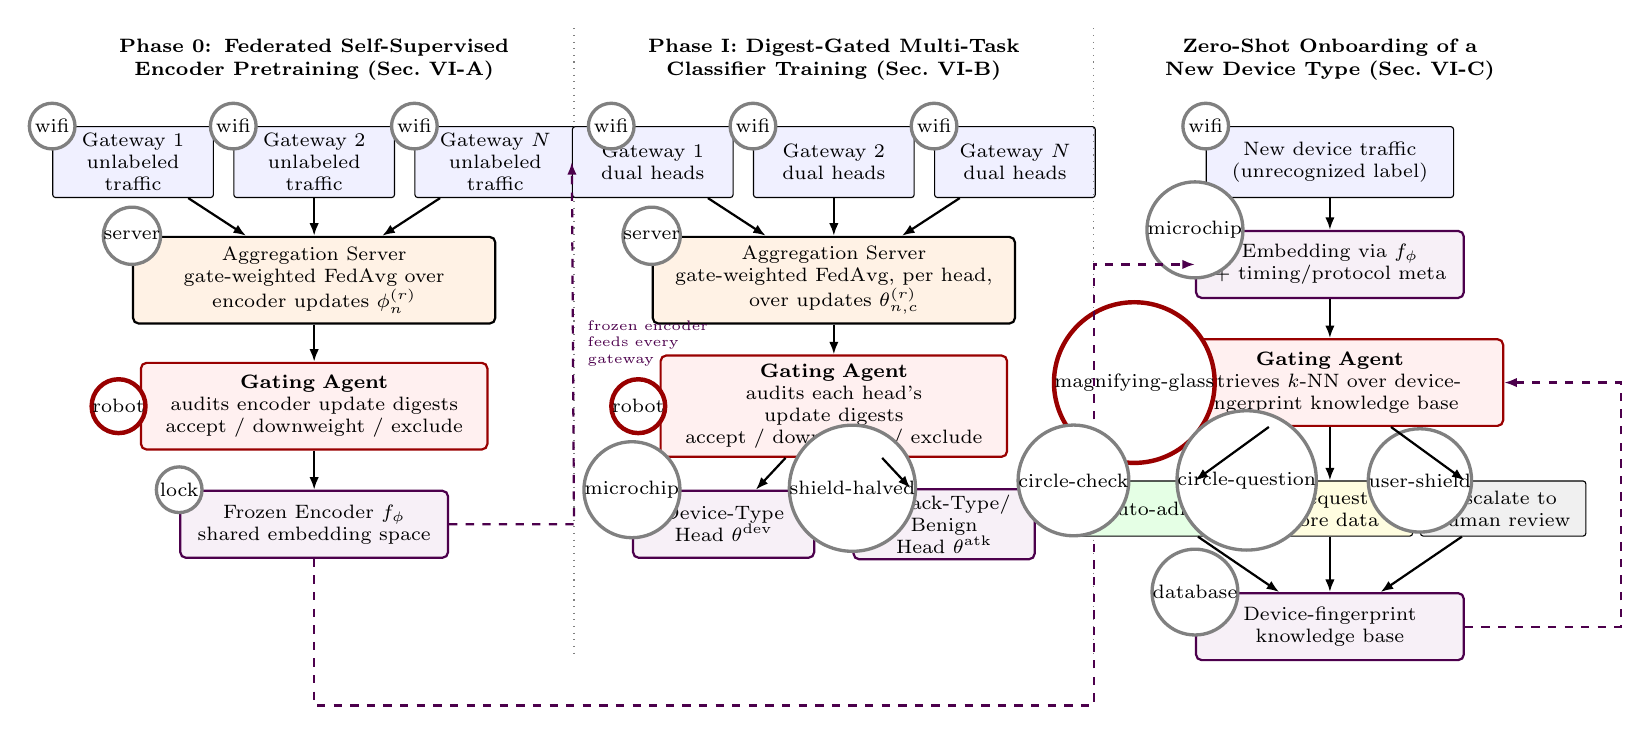
\begin{tikzpicture}[
    font=\scriptsize,
    gateway/.style={rectangle, draw, rounded corners=1pt, fill=blue!6,
        minimum width=2.0cm, minimum height=0.9cm, text width=1.9cm, align=center, inner sep=2pt},
    server/.style={rectangle, draw, thick, rounded corners=2pt, fill=orange!10,
        minimum width=4.6cm, minimum height=1.1cm, text width=4.3cm, align=center, inner sep=3pt},
    agent/.style={rectangle, draw=red!60!black, thick, rounded corners=2pt, fill=red!6,
        minimum width=4.4cm, minimum height=1.1cm, text width=4.1cm, align=center, inner sep=3pt},
    frozen/.style={rectangle, draw=violet!60!black, thick, rounded corners=2pt, fill=violet!6,
        minimum width=3.4cm, minimum height=0.85cm, text width=3.1cm, align=center, inner sep=2pt},
    head/.style={rectangle, draw=violet!60!black, thick, rounded corners=2pt, fill=violet!6,
        minimum width=2.3cm, minimum height=0.85cm, text width=2.0cm, align=center, inner sep=2pt},
    decision/.style={rectangle, draw, rounded corners=1pt, minimum width=2.1cm,
        minimum height=0.7cm, text width=1.9cm, align=center, inner sep=2pt},
    stagetitle/.style={font=\bfseries\scriptsize, align=center, text width=6.0cm},
    arr/.style={-{Latex[length=1.6mm]}, thick},
    dashedarr/.style={-{Latex[length=1.6mm]}, thick, dashed, violet!60!black},
    badge/.style={circle, draw=black!50, very thick, fill=white, minimum size=0.58cm, inner sep=0pt},
    agentbadge/.style={circle, draw=red!60!black, ultra thick, fill=white, minimum size=0.62cm, inner sep=0pt},
]

%% ================= Stage 1 (centered at x=0): Phase 0 =================
\node[stagetitle] (s1title) at (0,3.3) {Phase 0: Federated Self-Supervised Encoder Pretraining (Sec.~VI-A)};

\node[gateway] (g1a) at (-2.3,2.0) {Gateway 1\\ unlabeled traffic};
\node[gateway] (g1b) at (0,2.0)    {Gateway 2\\ unlabeled traffic};
\node[gateway] (g1c) at (2.3,2.0)  {Gateway $N$\\ unlabeled traffic};
\node[badge] at (g1a.north west) {\sysicon{wifi}};
\node[badge] at (g1b.north west) {\sysicon{wifi}};
\node[badge] at (g1c.north west) {\sysicon{wifi}};

\node[server] (srv1) at (0,0.5) {Aggregation Server\\ gate-weighted FedAvg over\\ encoder updates $\phi_n^{(r)}$};
\node[badge] at (srv1.north west) {\sysicon{server}};
\node[agent] (agent1) at (0,-1.1) {\textbf{Gating Agent}\\ audits encoder update digests\\ accept / downweight / exclude};
\node[agentbadge] at ([xshift=-0.27cm]agent1.west) {\sysicon{robot}};
\node[frozen] (frozenenc) at (0,-2.6) {Frozen Encoder $f_\phi$\\ shared embedding space};
\node[badge] at (frozenenc.north west) {\sysicon{lock}};

\draw[arr] (g1a) -- (srv1);
\draw[arr] (g1b) -- (srv1);
\draw[arr] (g1c) -- (srv1);
\draw[arr] (srv1) -- (agent1);
\draw[arr] (agent1) -- (frozenenc);

%% ---------- divider 1 ----------
\draw[dotted, gray] (3.3,3.7) -- (3.3,-4.3);

%% ================= Stage 2 (centered at x=6.6): Phase I =================
\node[stagetitle] (s2title) at (6.6,3.3) {Phase I: Digest-Gated Multi-Task Classifier Training (Sec.~VI-B)};

\node[gateway] (g2a) at (4.3,2.0) {Gateway 1\\ dual heads};
\node[gateway] (g2b) at (6.6,2.0) {Gateway 2\\ dual heads};
\node[gateway] (g2c) at (8.9,2.0) {Gateway $N$\\ dual heads};
\node[badge] at ([xshift=0.5cm]g2a.north west) {\sysicon{wifi}};
\node[badge] at (g2b.north west) {\sysicon{wifi}};
\node[badge] at (g2c.north west) {\sysicon{wifi}};

\node[server] (srv2) at (6.6,0.5) {Aggregation Server\\ gate-weighted FedAvg, per head,\\ over updates $\theta_{n,c}^{(r)}$};
\node[badge] at (srv2.north west) {\sysicon{server}};
\node[agent] (agent2) at (6.6,-1.1) {\textbf{Gating Agent}\\ audits each head's update digests\\ accept / downweight / exclude};
\node[agentbadge] at ([xshift=-0.27cm]agent2.west) {\sysicon{robot}};
\node[head] (devclf) at (5.2,-2.6) {Device-Type\\ Head $\theta^{\text{dev}}$};
\node[head] (atkclf) at (8.0,-2.6) {Attack-Type/\\ Benign Head $\theta^{\text{atk}}$};
\node[badge] at (devclf.north west) {\sysicon{microchip}};
\node[badge] at (atkclf.north west) {\sysicon{shield-halved}};

\draw[arr] (g2a) -- (srv2);
\draw[arr] (g2b) -- (srv2);
\draw[arr] (g2c) -- (srv2);
\draw[arr] (srv2) -- (agent2);
\draw[arr] (agent2) -- (devclf);
\draw[arr] (agent2) -- (atkclf);

\draw[dashedarr] (frozenenc.east) -- (3.3,-2.6) -- (g2a.west);
\node[font=\tiny, align=left, violet!60!black, anchor=west, text width=1.7cm] at (3.35,-0.3) {frozen encoder\\ feeds every\\ gateway};

%% ---------- divider 2 ----------
\draw[dotted, gray] (9.9,3.7) -- (9.9,-4.3);

%% ================= Stage 3 (centered at x=12.9): Onboarding =================
\node[stagetitle] (s3title) at (12.9,3.3) {Zero-Shot Onboarding of a New Device Type (Sec.~VI-C)};

\node[gateway, text width=3.0cm, minimum width=3.1cm] (newdev) at (12.9,2.0) {New device traffic\\ (unrecognized label)};
\node[badge] at (newdev.north west) {\sysicon{wifi}};
\node[frozen] (embnew) at (12.9,0.7) {Embedding via $f_\phi$\\ + timing/protocol meta};
\node[badge] at (embnew.north west) {\sysicon{microchip}};
\node[agent] (agent3) at (12.9,-0.8) {\textbf{Gating Agent}\\ retrieves $k$-NN over device-\\ fingerprint knowledge base};
\node[agentbadge] at ([xshift=-0.27cm]agent3.west) {\sysicon{magnifying-glass}};

\draw[arr] (newdev) -- (embnew);
\draw[arr] (embnew) -- (agent3);
\draw[dashedarr] (frozenenc.south) -- (0,-4.9) -- (9.9,-4.9) -- (9.9,0.7) -- (embnew.west);

\node[decision, fill=green!10] (admit) at (10.7,-2.4) {Auto-admit};
\node[decision, fill=yellow!12] (defer) at (12.9,-2.4) {Request\\ more data};
\node[decision, fill=gray!12] (escalate) at (15.1,-2.4) {Escalate to\\ human review};
\node[badge] at (admit.north west) {\sysicon{circle-check}};
\node[badge] at (defer.north west) {\sysicon{circle-question}};
\node[badge] at (escalate.north west) {\sysicon{user-shield}};

\draw[arr] (agent3) -- (admit);
\draw[arr] (agent3) -- (defer);
\draw[arr] (agent3) -- (escalate);

\node[frozen] (kb) at (12.9,-3.9) {Device-fingerprint\\ knowledge base};
\node[badge] at (kb.north west) {\sysicon{database}};
\draw[arr] (admit) -- (kb);
\draw[arr] (defer) -- (kb);
\draw[arr] (escalate) -- (kb);
\draw[dashedarr] (kb.east) -- (16.6,-3.9) -- (16.6,-0.8) -- (agent3.east);

\end{tikzpicture}
}
    \caption{System overview. The Gating Agent inspects each client's per-round digest before aggregation (center), a design validated across the federated encoder/classifier training loop and, using the same retrieval signal, at zero-shot device onboarding (right).}
    \label{system}
\end{figure*}

\section{Experimental Results}
\label{sec:results}
We evaluate on two real IoT datasets: N-BaIoT \cite{meidan2018nbaiot} (9 physical devices as 9 federated clients, benign/gafgyt/mirai) and CIC IoT-DIAD 2024 (9 clients, 8-class attack taxonomy), under 25-round federated training with $\alpha{=}3/9$ malicious clients unless noted, plus real UNSW device-identification traffic \cite{sivanathan2018classifying} for the device-type task. No dataset available to us provides both device-type and attack-type labels on the same traffic, so device identification and intrusion detection are evaluated as two independent poisoning experiments on the same shared-encoder Gating Agent design, not one model attacked on both tasks simultaneously -- we report this explicitly rather than let Fig.~\ref{system}'s shared architecture imply a joint experiment that was not run. Neither literature (Section \ref{sec:relwork}) tests either task's poisoning robustness, so we first establish this is not a hypothetical concern: plain FedAvg genuinely degrades under realistic poisoning for device identification just as for intrusion detection.

\subsection{Plain FL degrades under poisoning for both tasks it is asked to do}
On attack-classification, Table \ref{tab:robustness}'s FedAvg column shows the degradation directly: untargeted poisoning drops macro-F1 from 0.996 to as low as 0.139 ($\alpha{=}2$), and targeted poisoning succeeds at its actual objective (100\% success rate) at every $\alpha \geq 1$ -- plain FedAvg provides no defense at all against a targeted attacker regardless of how few clients are compromised.

The same is true for the task prior FL device-ID literature does not test: on real UNSW traffic (18 classes, $n{=}10$ clients, identical threat model \cite{bagdasaryan2020backdoor}), Table \ref{tab:deviceid-robustness} shows device-type macro-F1 collapsing under untargeted poisoning -- 0.828 to 0.038 at $\alpha{=}4$, more severely than attack-classification above. The targeted attacker succeeds unevenly -- 0.63 success at $\alpha{=}2$ but 0.0 at $\alpha{=}3$, where accuracy has already collapsed enough (0.249) that the source class is barely predicted at all -- reported as observed, not smoothed. Prior FL device-ID work \cite{chen2025confeddi,wang2025fgliot,he2021edge} reports no poisoning evaluation at all; the one paper that does \cite{sanchez2021robust} uses a different, non-network-traffic task. To our knowledge this is the first poisoning-degradation measurement for network-traffic-based federated device-type classification.

\begin{table}[t]
\centering
\small
\caption{UNSW device-identification robustness: plain FedAvg, no defense.}
\label{tab:deviceid-robustness}
\begin{tabular}{@{}ccc@{}}
\toprule
$\alpha$ & \textbf{Untargeted (macro-F1)} & \textbf{Targeted (F1; success rate)} \\
\midrule
0 & 0.828 & 0.828; 0.02 \\
1 & 0.581 & 0.851; 0.02 \\
2 & 0.220 & 0.768; 0.63 \\
3 & 0.073 & 0.249; 0.00 \\
4 & 0.038 & 0.069; 0.73 \\
\bottomrule
\end{tabular}
\end{table}

\subsection{A rule-based reference confirms the design, but has real limits}
Table \ref{tab:robustness} compares a rule-based Gating Agent (fixed thresholds, same digest and posterior) against plain FedAvg, trimmed-mean, and Krum on N-BaIoT. It tracks Krum reasonably well against untargeted attacks, far above plain FedAvg, but provides little defense against targeted attacks past $\alpha{=}2$ (success rate reaches 1.00, matching FedAvg), since it only inspects an aggregate digest.

\begin{table}[t]
\centering
\small
\caption{N-BaIoT robustness: macro-F1 (targeted also reports success rate).}
\label{tab:robustness}
\begin{tabular}{@{}ccccc@{}}
\toprule
$\alpha$ & \textbf{FedAvg} & \textbf{Trim.} & \textbf{Krum} & \textbf{Gating (rule)} \\
\midrule
\multicolumn{5}{@{}l}{\textit{Untargeted (macro-F1)}} \\
0 & 0.996 & 0.997 & 0.992 & 0.997 \\
1 & 0.927 & 0.996 & 0.992 & 0.992 \\
2 & 0.139 & 0.214 & 0.996 & 0.954 \\
3 & 0.357 & 0.524 & 0.992 & 0.320 \\
4 & 0.185 & 0.174 & 0.998 & 0.944 \\
\multicolumn{5}{@{}l}{\textit{Targeted (macro-F1; success rate)}} \\
1 & 0.545;1.0 & 0.997;.0 & 0.992;.0 & 0.807;.5 \\
2 & 0.544;1.0 & 0.548;1.0 & 0.996;.0 & 0.546;1.0 \\
3 & 0.174;1.0 & 0.525;1.0 & 0.992;.0 & 0.525;1.0 \\
4 & 0.174;1.0 & 0.179;1.0 & 0.998;.0 & 0.194;1.0 \\
\bottomrule
\end{tabular}
\end{table}
At $\alpha{=}3$ untargeted, a 5-seed re-run (0.320, 0.142, 0.984, 0.152, 0.174) shows this cell is genuinely bimodal, not merely noisy, reported rather than smoothed over. Krum is the strongest defense throughout; the rule-based agent's real limitation is judging only an aggregate digest.

Against trust-building at $D{=}10$, an ablation isolates the long-term posterior's contribution: 0.986 macro-F1 with it, 0.185 with the identical digest but the posterior never consulted -- the round-level digest alone is nearly useless once an attacker has built 10 rounds of clean-looking history.

\subsection{The real LLM Gating Agent: failure, diagnosis, and a fix that works}
Testing the actual LLM-based agent against the trust-building attack, four independently-motivated 8B (Llama 3.1) configurations -- single-turn, an optional history tool, and a hybrid external-trust architecture -- all landed between \textbf{0.174 and 0.251} macro-F1 at $D{=}10$, far below the rule-based reference. Every configuration showed the same symptom: no benefit of the doubt for a long clean history against one anomalous-looking round.

Per-round decision logging traced this to three fixable causes: a round-0 artifact, early-training volatility misread as anomalous, and a trust posterior with no recovery path once wrongly excluded. Fixing these closed only part of the gap (0.241 $\to$ 0.287), and exposed two more: a placeholder calibration-loss signal the model still cited, and a raw cosine value judged against one fixed anchor. The fix: cosine as a same-round z-score against other clients, and calibration-loss direction in words instead of a signed number the model sometimes misread.

On five hand-built test cases, Llama 3.1 8B still failed even with this fix -- it compared the two z-scores to each other rather than judging each against zero. A 14B model (Qwen2.5) got all five right. The full result: \textbf{0.9041} macro-F1 at $D{=}10$ with zero fallback rounds -- the first result to beat the rule-based reference (0.758).

\begin{table}[t]
\centering
\footnotesize
\caption{Qwen2.5 14B Gating Agent, real poisoning attacks, both datasets.}
\label{tab:headline}
\begin{tabular}{@{}lccc@{}}
\toprule
\textbf{Config} & \textbf{F1} & \textbf{Fallback} & \textbf{Rule} \\
\midrule
CIC, TB $D{=}10$ (3 seeds) & 0.896--0.912 & 0/25 & 0.758 \\
CIC, TB $D{=}20$ & 0.898 & 0/25 & -- \\
CIC, untargeted & 0.912 & 0/25 & -- \\
CIC, targeted & 0.907 & 0/25 & -- \\
NB, TB $D{=}10$ (3 seeds) & 0.995--0.997 & 0/25 & 0.99 \\
NB, TB $D{=}0/20$ & 0.996/0.996 & 0/25 & .32/.99 \\
NB, untargeted/targeted & 0.996/0.997 & 0/25 & -- \\
\bottomrule
\end{tabular}
\end{table}

This result is not a lucky configuration. Table \ref{tab:headline} shows all thirteen configurations -- three seeds on each dataset's flagship trust-building config, two delay values beyond that, three attack types, two structurally different real datasets -- landing in a tight band with zero fallback rounds and, wherever a targeted-attack success rate applies, under 1\%: the attack fails at its actual objective, not just at tanking aggregate accuracy. N-BaIoT's own 3-seed replication (0.9954, 0.9971, 0.9974) is as tight as CIC IoT-DIAD's, closing the one asymmetry in seed coverage between the two datasets.

\subsection{A measured capability boundary}
Applying the identical fix to Llama 3.1 8B on the single-turn architecture reached only \textbf{0.1375} macro-F1 -- malicious and honest clients receive nearly identical decisions from round 19 onward. None of four 8B attempts approached the 14B result. This is consistent with recent findings that small language models lag on judgment tasks even when general reasoning is comparable \cite{laddha2026slmjury,bi2025judgeboard}; to our knowledge this gap was not previously measured for federated poisoning-defense trust judgment. For the tested model families and prompt design, 14B parameters or more is required; the tested 8B configuration is not a substitute.

Is 14B a floor or a ceiling? qwen2.5:32b on the identical $D{=}10$ configuration reached \textbf{0.9964} against 14B's 0.9974 -- statistically indistinguishable -- while taking 2.7$\times$ longer (2277s vs.\ 854s). Going bigger bought no accuracy and cost more compute: 14B already behaves like a ceiling, not a floor, though this is bounded to the Qwen2.5 family and prompt tested, not a general scaling law.

One of those four attempts -- offering a FetchHistory tool call before deciding -- made things categorically worse: with the option present, the 8B model gave \emph{every one of 5 synthetic test cases} the identical "downweight" verdict, never once invoking the tool (0/5). Removing only the tool-offering sentence restored correct discrimination. A control with the same background text but no tool option discriminates fine -- merely offering a third, structurally different response shape collapses the model's output toward one non-committal action, even when the hatch is never taken.

\subsection{Honest comparison to a fast non-LLM baseline}
We built a lightweight version of GShield \cite{sameera2025gshield}: PCA-reduce each round's updates, 2-means cluster, exclude any client whose distance from the larger cluster is an outlier. It reaches 0.914--0.921 on CIC IoT-DIAD and 0.995--0.997 on N-BaIoT -- matching or exceeding the LLM Gating Agent, at 17--34 seconds versus 15--45 minutes. We claim no accuracy win; the LLM's advantage is that every exclusion carries a rationale, which a distance threshold cannot provide.

An attacker blending its update toward its own clean-label gradient for stealth \cite{bagdasaryan2020backdoor} fools the clustering at high blend strength (2 of 3 malicious clients land in "benign"), but the same blend that evades detection also dilutes the damage -- the aggregate outcome barely moves for either defense.

Direction-blending evades norm and cosine but never targeted the digest's third signal. A calibration-aware variant that also searches blend strength to minimize the attacker's own measured calibration impact found no additional edge (F1 0.997--0.998, N-BaIoT): calib\_loss\_delta is judged as a same-round, cross-client z-score, so minimizing only its own impact still lands as an outlier (z up to 61) against honest clients it cannot see. Pooling this estimate across colluding malicious clients halves their exclusion rate (26/75 to 14/75) but still finds no edge (F1 0.997--0.998): the blend strength stealth requires dilutes the attack too much to matter even on rounds that still get caught.

\subsection{Making the LLM selective closes most of the cost gap}
If the LLM's real value is the rationale, not raw accuracy, it should only be invoked where a rationale is decision-relevant, not every round. We built a cheap admission filter from infrastructure we already have -- the same digest z-scores and thresholds the rule-based policy uses, applied only to decide whether the LLM is called. A client whose update norm, cosine similarity, and calibration loss are all comfortably normal (with a safety margin short of the downweight threshold) is accepted deterministically, for free; every other client gets the identical hybrid LLM judgment. This is not GShield's clustering mechanism; it reuses our own digest as a pre-filter instead.

The first version had a real failure worth reporting, not hiding: on N-BaIoT it matched full-LLM accuracy while cutting calls to 41--53\%, but on CIC IoT-DIAD's longest delay ($D{=}20$), macro-F1 collapsed to \textbf{0.1869} against a 0.898 reference. Per-round inspection traced it precisely: the fast path always writes a perfect, noiseless 1.0 to the trust posterior, building more trust for a patient 20-round attacker than the real LLM's noisier judgments would have -- so the long-term override fired every attack round, permanently downgrading exclude to downweight, and the model never recovered. The fix: the posterior updates only from genuine LLM judgments, never the fast path, so an unaudited shortcut cannot manufacture more trust than a real judgment would grant.

With this fix, all 11 configurations across both datasets match or slightly exceed full-LLM accuracy (0.9966--0.9980 on N-BaIoT; 0.906--0.921 on CIC IoT-DIAD, including 0.9173 on the previously-broken case) while calling the LLM for only 33--52\% of decisions -- roughly halving the full-LLM cost without giving up accuracy. This does not close the 50--100x gap to GShield's 17--34 seconds, but the failure it took to get here is itself evidence for the paper's claim: an unaudited shortcut can quietly undermine the exact trust mechanism it supports, which an LLM's rationale is supposed to let a human catch.

Grounding this in real instrumentation rather than aggregate totals (N-BaIoT, $D{=}10$, 216 decisions; Table \ref{tab:resource}): the fast path carries no measurable inference cost at all (Welch's $t{=}114.7$, $p<10^{-100}$). The 14B model holds a fixed $\sim$9.6\,GB memory footprint regardless of path taken; unlike \cite{jamshidi2026thinkfast}'s wattmeter setup, we report no energy figure, since none was available and estimating one would not be honest.

\begin{table}[t]
\centering
\scriptsize
\caption{Real per-decision latency/CPU, selective-LLM policy (N-BaIoT).}
\label{tab:resource}
\begin{tabular}{@{}lccc@{}}
\toprule
\textbf{Path} & \textbf{n} & \textbf{Latency (s)} & \textbf{CPU (\%)} \\
\midrule
Fast path & 119 & 0.00005 $\pm$ 0.00004 & 0.0 \\
LLM call & 97 & 3.75 $\pm$ 0.32 & 13.9 $\pm$ 2.9 \\
\bottomrule
\end{tabular}
\end{table}

The fast path is itself a new attack surface -- an update crafted to look "comfortably normal" gets no LLM scrutiny. Re-running the constrain-and-scale attacker against it ($\lambda\in\{0, 0.9, 0.99\}$, targeted, CIC IoT-DIAD), the same blending that lands 2 of 3 malicious clients in GShield's "benign" cluster never once enters the fast path's normal band (0/75); F1 (0.917--0.919) and targeted success ($\leq$1.1\%) stay flat. A coordinated variant -- pooling clean gradients into one shared reference -- fares no better: GShield (0.918--0.921) and the selective-LLM policy (0.917--0.920, bypass still 0/75) are both unmoved.

\subsection{Generalization: unseen attack shapes and a new dataset}
A skeptical reading of every result so far is that the agent pattern-matches its calibration exemplars rather than reasoning about anomaly generally, and that the round-relative digest's claimed deployment-agnosticism has never actually been tested across deployments. We tested both, with the prompt and thresholds completely unmodified (Table \ref{tab:generalization}): three attack shapes unlike anything in the calibration exemplars (\textbf{slow-drip}: strength ramps over 20 rounds instead of switching on; \textbf{intermittent}: attacks only every third round; \textbf{free-rider}: submits no real update at all -- not poisoning, a distinct FL threat of shirking contribution while still being counted), on N-BaIoT; and the identical selective-LLM policy transferred, with zero recalibration, to real CIC IoT 2023 data (39 features vs.\ 115/118 for the other two datasets, never used for this agent before), across three attack types.

\begin{table}[t]
\centering
\scriptsize
\caption{Generalization tests, prompt and thresholds unchanged throughout.}
\label{tab:generalization}
\begin{tabular}{@{}lccl@{}}
\toprule
\textbf{Test} & \textbf{Undef.} & \textbf{Gated} & \textbf{Note} \\
\midrule
Slow-drip (NB) & 0.185 & 0.997 & ramps over 20 rounds \\
Intermittent (NB) & 0.138 & 0.997 & every 3rd round \\
Free-rider (NB) & 0.995 & 0.997$^\dagger$ & idle, not poisoning \\
CIC'23, TB $D{=}10$ & -- & 0.691 & vs.\ 0.686 no-atk ceiling \\
CIC'23, untargeted & -- & 0.685 & zero recalibration \\
CIC'23, targeted & -- & 0.688 & 20\% success (unresolved) \\
\bottomrule
\end{tabular}
\\[2pt]
{\scriptsize $\dagger$ Only after a fix -- see text.}
\end{table}

Both damaging new shapes are fully defended, matching the flagship numbers the agent was calibrated against. Free-riding barely hurts undefended accuracy, and the first gated result looked identical -- until per-round inspection found free-riders got "accept" every round: the fast-path filter and the LLM's calibration examples were one-sided, catching anomalously \emph{large} update norms but never anomalously \emph{small} (idling) ones. We fixed both halves: the fast-path check became symmetric ($|z|>\tau$ instead of $z>\tau$), and a fourth calibration example now teaches the negative-z case. Re-tested: every free-rider round now resolves to downweight/exclude, and the flagship N-BaIoT $D{=}10$ config still gets F1$=$0.9974 -- no regression, at a small honest cost (LLM-call fraction 44.9\%$\to$51.4\%).

On CIC IoT 2023, the three attack types land at 0.685--0.691 -- well below 0.90+ elsewhere, but an undefended, no-attacker run on the same data also gets 0.686. This simpler 39-feature representation has a lower natural ceiling, and the agent absorbs the attacks' impact regardless of dataset. One caveat: targeted-success rate here is 20\% vs.\ under 1\% elsewhere, plausibly because this dataset's classes are more confusable in 39 dimensions -- a hypothesis, not confirmed.

\subsection{The same agent design, validated on two more decisions}
The same design applies to three decisions: round-wise gating (above), zero-shot device onboarding, and intrusion triage. Onboarding correctly deferred a genuinely unseen device (75\% confidence) and auto-admitted a known one (97\%). Triage found a genuine limitation: of 37 real N-BaIoT misclassifications, \textbf{0 were flagged as likely false positives} -- confident, in-distribution confusions, not the anomalies the signal was designed to catch. A signal-design gap, not a reasoning failure.

\subsection{Closing two deployment gaps directly}
Rather than leave graceful degradation and concept-drift adaptation as stated gaps, we fixed and tested both. An opt-in wrapper falls back to the rule-based policy on an unreachable LLM backend; verified against a real outage (Ollama killed mid-run), training continued without crashing at F1$=$0.9972. For drift, a naive EWMA baseline failed once tested (100\% false positives, since once flagged it stops updating); the fix reuses the same cross-client z-score trick used for update-norm/cosine, cutting the false-positive rate from 91\% to 24\% under synthetic drift -- not perfect, reported rather than resolved.

\section{Conclusion}
We validated a real LLM-based Gating Agent for federated IoT poisoning defense, on a task no prior work evaluates together and that genuinely degrades under poisoning. The design matches a fast non-LLM baseline's accuracy rather than beating it, so we position its contribution honestly: auditable, rationale-backed decisions, a selective variant halving LLM-call cost, a measured 8B-vs-14B-vs-32B capability boundary, generalization to unseen attack shapes and a new dataset, and no edge for independent or colluding adaptive attackers. We closed two deployment gaps directly rather than leaving them as future work. Remaining limitations: attacks are simulated, not live against real hardware; the LLM pool is entirely local, blocked on API credits for a hosted-frontier-model test.

\bibliographystyle{bibliography/IEEEtran}
\bibliography{bibliography/IEEEabrv,bibliography/IEEEexample}

\end{document}
